\section{Методы исследования кристалличности}

Оценить степень кристалличности можно, используя различия между разнообразными характеристиками амофрной и кристаллической фаз.
Приведем основные методы, с помощью которых изучается кристалличность \cite{cryst3}.

\subsection{Плотность}

Самое простое различие между фазами -- плотность. При точности измерения < 0.1 кг/м3 и аддитивности по массе степень кристалличности будет определяться как
\[
\%_{x_{\nu}} =\frac{\rho - \rho_a}{\rho_c-\rho_a}
\]
Плотность кристаллической фазы расчитывается из параметров базисной клетки. Плотность аморфной фазы может быть получена экстраполяцией удельного объема, измеренного для расплава при разных температурых методами дилатометрии. Плотности также могут быть определены экспериментально, экстраполяцией значений плотности образцов с известной кристалличностью. Такие измерения требуют предварительной калибров другими методами, такими как рентгеноструктурный анализ.

\subsection{Термический анализ}
Поскольку кристаллические области при нагреве плавятся, а аморфные нет, теплота плавления может быть исопльзована как мера степени кристалличности.
Эта энергия может быть измерена с использованием дифференциальной сканирующей калориметрии (ДСК). В ДСК измеряется количество теплоты, поглощаемое или выделяемое образцом, по сравнению с эталоном (пустой тигель) во время термических переходов при постоянной скорости нагева (охлаждения), в изотермических условиях, как функция от времени.

Массовая доля кристаллической фазы, таким образом, может быть определена из измеренной  теплоте плавления ($\Delta H_m$) и известного значения для полностью кристаллического материала $\Delta H^0_m$. При использовании этого метода , однако, встречаются трудности при работе с полимерами с низкой степенью кристалличности. Помимо этого, для корректного расчета степени кристалличности требуется тщательная оценка фоновой поправки.

\subsection{Спектроскопия}
ИК-спектроскопия, раманоское рассеяние и ЯМР -- три широко распространенных спектроскопических метода, используемые для анализа структурных характеристик, таких как конформация, стереорегулярность, ориентация, внутри- и межмолекулярные взаимодействия полимеров. Эти техники также используются для определения кристалличности, после калибровки с другими методами, такими как измерение плотности или рентгеновская дифракция.

На структурном урвоне, конформация полимерных цепей в кристаллических и аморфных областях различна. Поэтому, спектроскопические методы, такие как ИК и рамановская спектроскопия могут применяться для исследования кристаллизации, в случае, если полосы поглощения кристалличных и аморфных конформаций легко различимы.

Благодаря различию между подвижностью молекул в аморфных и кристаллических регионах, твердотельная спектроскопия ЯМР тоже может быть использован для характеристики кристалличности полимеров.


\subsection{Микроскопия}
Более крупные структуры, такие как сферолиты, сформированные из ламелей и фибрилл, можно изучать методами оптический микроскопии, например поляризационной микроскопией.


\subsection{Дифракция}

Наконец, полимерные цепи упакованы в кристаллические решетки, и эти решетки, даже будучи неупорядоченными друг относительно друга, порождают кристаллические дифракционные пики в экперименте по широкоугловому рассеянию (WAXS -- Wide-Angle X-ray Scattering). Таким образом, интенсивность пиков рентгеновской дифракции может быть использована в качестве \textit{прямого} измерения степени кристалличности полимеров. Вдобавок, во время кристаллизации полимер часто образует и структуры большего масштаба, такие как  фибриллы. Эти более крупные структуры можно наблюдать, используя малоугловое рассеяние (SAXS -- Small-Angle X-Ray Scattering) и электронную микроскопию. По картинам SAXS, таким образом, можно судить об эффекте изменений в кристалличности на морфологию полимера.


Как видно из описания методов, в разных методиках измерений за кристалличность принимаются разные величины. Когда это возможно, кристалличность рекомендуется измерять посредством рентгеноструктурного анализа. 


\subsection{Картография кристалличности}
При изучении степени кристалличности обычно подразумевается, что кристаллиты распределены по образцу равномерно. Это далеко не всегда так. Неоднородность внешних условий (например, градиент температур) в процессе 3D-печати приводит также и к появлению градиентов кристалличности в конечном изделии. 
Такие неоднородности могут быть обнаружены сканирующими техниками ИК, рамановской или терагерцовой спектроскопии (\cite{thz})  с разрешением $\sim 100$ мкм, или с помощью микрофокусной дифракции и дифракции под скользящими углами(для изучения поверхностных слоев материала), примерно с таким жже разрешением, а также  Среди этих техник выделяется нанофокусная дифракция, дающая разрешение около 1 мкм.
Составление подобных карт важно для понимания влияния параметров процесса, таких как температура, скорость охлаждения, на характеристики изготовленных изделий.



\section{Рентгеноструктурный анализ полимеров}
Большая часть сведений и иллюстраций в данном разделе взята из пособия \cite{2d-diff}.

При упругом рассеянии рентгеновского излучения на полимерах упорядоченно уложенные фракменты цепей будут порождать узкие кристаллические пики при определенных углах рассеяния. 
Соотношение между углом рассеяния $2\theta$ и расстоянием между плоскостями в кристалле определяется законом Брэгга:
\[
\lambda = 2d_{hkl} \sin \Theta,
\]
где $d_{hkl}$ -- геометрическая функция формы и размера базисной клетки.
В свою очередь, неупорядоченные цепи, с ближним порядком по типу жидкости, порождают широкое аморфное гало. При рассеянии на газах получаются обычные профили рассеяния, без признаков дифракции (рис. \ref{fig:scattering}).

\begin{figure}
    \centering
    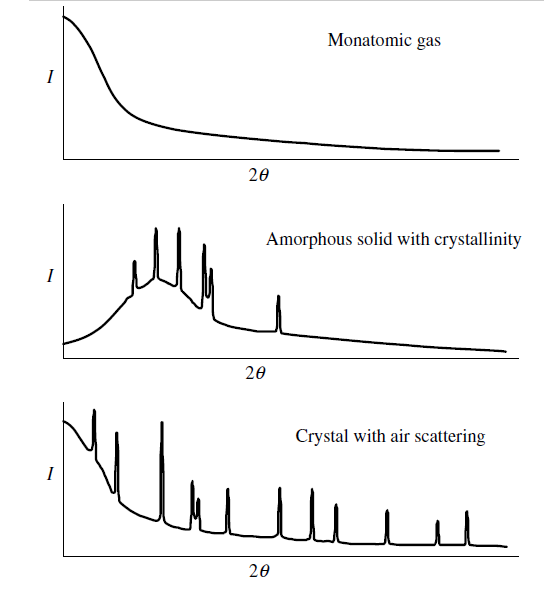
\includegraphics[width = \linewidth]{fig/scattering.PNG}
    \caption{Картины рассеяния рентгеновских лучей на газе (сверху), частично-кристаллическом материале (по центру) и кристаллическом материале в присутствии воздуха (снизу)}
    \label{fig:scattering}
\end{figure}

Положение дифракционных пиков иногда выражается через вектор рассеяния \textbf{q}, где $q = 2\pi/d = 4\pi \sin \theta / \lambda$. 

В образцах с неориентированными кристаллическими доменами, в приближении двухфазной модели степень кристалличности будет определяться как 

\[
X_m = \frac{\int_0^{\infty} q^2 I_c(q) dq}{\int_0^{\infty} q^2 I(q)(q)] dq,}
\]
где $I_c(q)$ - интенсивность кристаллических пиков, $I(q)$ - суммарная интенсивность рассеяния.
При обработке реальных данных интегрирование, как правило, проводится в пределах q от 0.5 до 3 \AA.

\section{Материалы}

		
	\begin{figure}[h]
	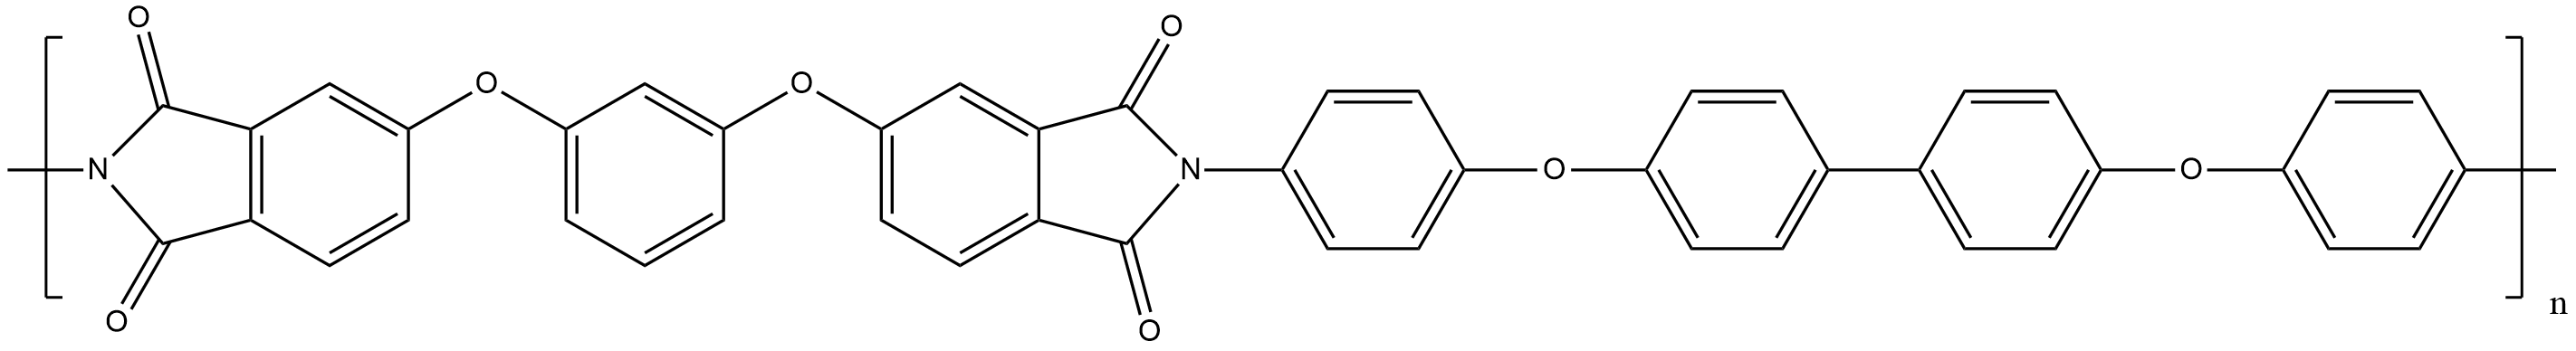
\includegraphics[width=\textwidth]{fig/formula.png}
	\caption{Структура полимера Р-ОДФО \cite{pi-formula}}
	\label{fig:formula}
	\end{figure}

Для исследования взяты образцы порошка Р-ОДФО и пленки, полученные на лазерной установке методом СЛС. Ранее исследованные свойства\cite{vaganov}:
 $T_g = 200$ \textdegree C, $T_m = 318$ \textdegree C, кристалличность оцененная из термического анализа -- 50\%.

Характеристики пленок после спекания (мощность лазера 65 Вт):
прочность на разрыв $ \sigma =36.80 \pm 2.51$ МПа, модуль упругости при растяжении   $ E = 1321 \pm 87$ МПа , максимальная деформация $ \varepsilon = 5.67  \pm 0.89$ \%. 


\section{Оборудование и схема эксперимента}
Установка, на которой проводился сканирующий эксперимент, расположена на синхротронной линии ID13 Европейского центра синхротронного излучения (ERSF) в Гренобле, Франция. Ее схема  изображена на рис. \ref{fig:experiment}. 

\begin{figure}[h]
    \centering
    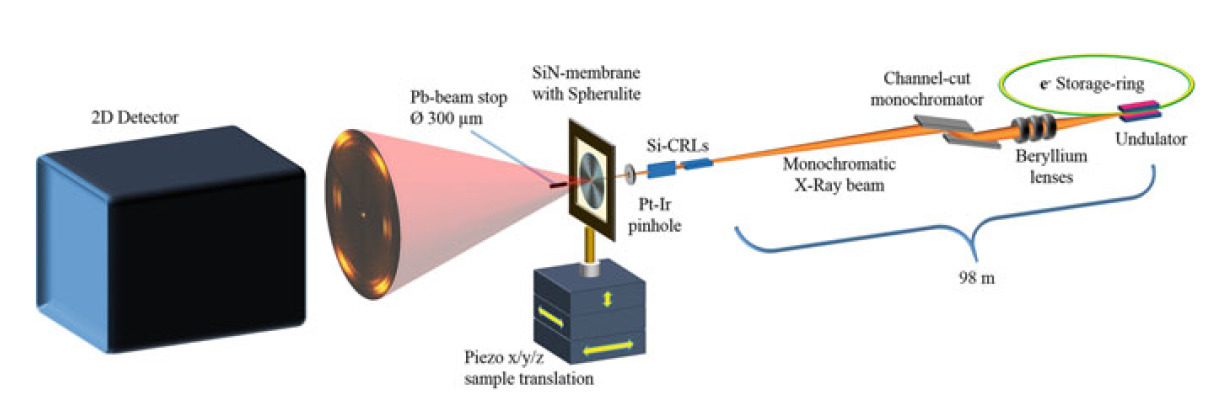
\includegraphics[width=\linewidth]{fig/ust.PNG}
    \caption{Экспериментальная установка. \cite{experiment}}
    \label{fig:experiment}
\end{figure}

\paragraph{Источник излучения}

	\begin{wrapfigure}[10]{r}{0.4\linewidth}
\singlespacing
\vspace{-5px}
%  \begin{center}
    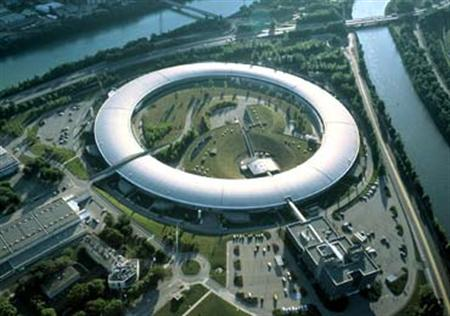
\includegraphics[width=\linewidth]{fig/pribor-photo.jpg}
    \vspace{3px}
    \caption{Синхротрон}
    \label{fig:ring}
%  \end{center}
\end{wrapfigure}

 Пучок рентгеновского излучения генерируется электронами, ускоренными до 6,3 ГэВ, которые проходят через ондулятор, расположенный внутри накопительного кольца. Затем рентгеновский луч белого спектра предварительно фокусируется на расстоянии около 98 м от накопительного кольца с использованием набора бериллиевых линз. Затем, с помощью монохроматора на основе монокристаллического кремния получают монохроматически пучок энергией $\approx 15$ кэВ ($\lambda = 0.835$ \AA) Конечная фокусировка луча в точке, близкой к положению образца, реализуется с использованием композиционных преломляющих линз на основе кремния, обеспечивающих размеры пучка в диапазоне 40-150 нм, в зависимости от предварительной фокусировки. Типичные значения потока фотонов в описанном режиме фокусировки составляют около $10^10$ фотонов в секунду, что дает плотности потока фотонов около $2,8\cdot 10^6$ фот$sdot$c$^{-1} \cdot$нм$^{-2}$. Размер рентгеновского пучка, использованного в данной работе, составляет около 200 нм по обеим координатам, шаг сканирования по обеим координатам составляет 1 мкм. 
 
 
Все это позволяет в итоге получить необходимую пространствннно-разрешенную информацию о структуре образцов.

 Чувствительный двумерный детектор  рентгеновского излучения от прямого пучка защищает свинцовая заслонка, которую можно видеть и на дифрактограммах (рис. \ref{fig:difractogram}).

Движение образца по осям x,y,z  с нанометровой точностью осуществляется с помощью сочетания так называемого гексапода и специально разработанного комплекса пьезо-приводов.

Калибровка, учитывающая  геометрию эксперимента и прочие факторы, а также азимутальное интегрирование производилось с помощью программного пакета pyFAI \cite{pyfai}, 



